\documentclass[]{article}

\usepackage{graphicx}
\usepackage{longtable}
\usepackage{hyperref}
\usepackage{color}
\usepackage{soul}
\usepackage{amsmath}


\DeclareRobustCommand{\hlcyan}[1]{{\sethlcolor{cyan}\hl{#1}}}
\DeclareRobustCommand{\hlgreen}[1]{{\sethlcolor{green}\hl{#1}}}
\DeclareRobustCommand{\hlred}[1]{{\sethlcolor{red}\hl{#1}}}
\DeclareRobustCommand{\hlyellow}[1]{{\sethlcolor{yellow}\hl{#1}}}
\DeclareRobustCommand{\hlorange}[1]{{\sethlcolor{orange}\hl{#1}}}


%opening
\title{Session 2}
\author{Fakhir}

\begin{document}

\maketitle

\section*{Solutions}

Break the function into two pieces, namely for $x>0$ and $x<0$. 

\[
f'(x)= 
\begin{cases}
1, & \text{if } x>0 \\
-1,& \text{if } x<0 \\
undefined, & \text{if } x=0
\end{cases}
\]

The reason it is undefined at $x=0$ is because $\Delta x$ can have one end on one piece of the function and the other end on different piece of the function. This implies that even if $\Delta x$ has same magnitude in different cases but its slope can drastically vary depending on how we choose the end points, as shown in the following figure:

\begin{center}
	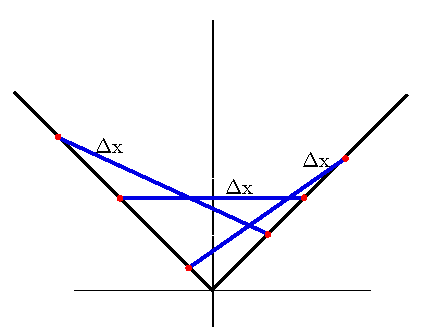
\includegraphics[scale=1]{images/section1_1}
\end{center}

\hlred{The above explanation may not be correct.} \\~\\

The arguments given in the MiT's solution appear to be much more convincing.

\end{document}
